\documentclass{beamer}

\documentclass{beamer}
\usepackage[utf8]{inputenc}
\usepackage[ngerman]{babel}
\usepackage{url}
\usepackage{xcolor}

\usetheme[compress]{Berlin}
\setbeamerfont{headline}{size=\large}
\setbeamerfont*{section in head/foot}{size=\tiny}
\setbeamertemplate{toc}{circle}
\setbeamertemplate{itemize subitem}[triangle] % if you want a triangle
\setbeamercovered{transparent}

\definecolor{myBlue}{rgb}{0,0.55,0.8}
\usecolortheme[named=myBlue]{structure}

\title{Das \LaTeX-KBS}
\subtitle{\small Grundlagen von \LaTeX, Ti\textit{k}Z und Co.}
\author
{
	Walter Stieben \texttt{\href{mailto:4stieben@informatik.uni-hamburg.de}{4stieben@inf}}\\
	\href{http://hauke-stieler.de/}{Hauke Stieler} \texttt{\href{mailto:4stieler@informatik.uni-hamburg.de}{4stieler@inf}}
}
\date{\footnotesize 12.01.2016}

\begin{document}
	\maketitle
	\tableofcontents\newpage
	\section{Was ist \TeX{} und \LaTeX{}}
		\subsection*{asd}
		\begin{frame}{Was ist \LaTeX{}}
			\textbf{\LaTeX{} und \TeX{}:}
			\begin{itemize}
				\item \TeX{} ist ein Textsatzsystem von Donald E. Knuth
				\item \LaTeX{} ist ein Satz von Makros für \TeX
				\item WYSIWYT (What You See Is What You Type)
			\end{itemize}
			\vspace{0.2cm}
			\textbf{Vorteile von \LaTeX{}:}
			\begin{itemize}
				\item Ergebnis sieht hübsch aus
				\item \LaTeX{} kümmert sich um die Formatierung
				\item Der Quelltext lässt sich Versionsverwalten
				\item Für mathematische Formeln sehr gut
				\item ``Ich möchte X mit \LaTeX{} machen'' $\rightarrow$
				Suchmaschine: ``latex X'' eingeben $\rightarrow$
				Ergebnis in den Quelltext kopieren
			\end{itemize}
		\end{frame}
\end{document}

\usepackage{siunitx}
\usepackage{physics}
\usepackage{chemfig}
\usepackage[siunitx]{circuitikz}
\usepackage{algorithmic}
\usepackage{mathtools}
\usepackage{environ}
%\usepackage{banyan-net}
%\usepackage{hypercube-5D}
\usepackage{tikz}
\usepackage{pgf}

\usetikzlibrary{
	arrows,
	automata,
	calc,
	intersections,
	hobby,
	petri,
	positioning,
	through
}

\title{\LaTeX{} advanced}
\subtitle{\small Ti\textit{k}Z, etc.}

\date{\footnotesize \today}

% Auskommentieren, um tikzpicture temporär zu deaktivieren:
% \RenewEnviron{tikzpicture}[1][]{\par\texttt{tikzpicture}\par}

\begin{document}
	\maketitle

	%%%%%%%%%%%%%%%%%%%%%%%%%%%%%%%%%%%%%%%%%%%%%%%%%%%%%%%%%%%%%%%%%%%%%%%

	\begin{frame}
		\begin{center}
			Danke Henning (\texttt{8pridoeh}) dass wir deine Folien aus dem WS14/15 benutzen dürfen :D
		\end{center}
		Und auch Danke an alle, die zu den Folien und zum Vortrag beigetragen haben:
		\begin{itemize}
			\item Walter Stieben \texttt{\href{mailto:4stieben@informatik.uni-hamburg.de}{4stieben@inf}}\\
			\item Ruben Felgenhauer \texttt{\href{mailto:4felgenh@informatik.uni-hamburg.de}{4felgenh@inf}}\\
			\item Malte Hamann \texttt{\href{mailto:1hamann@informatik.uni-hamburg.de}{1hamann@inf}}\\
			\item Hauke Stieler \texttt{\href{mailto:4stieler@informatik.uni-hamburg.de}{4stieler@inf}}
		\end{itemize}
	\end{frame}
	
	%%%%%%%%%%%%%%%%%%%%%%%%%%%%%%%%%%%%%%%%%%%%%%%%%%%%%%%%%%%%%%%%%%%%%%%
	
	\begin{frame}
		\tableofcontents[hideallsubsections]
	\end{frame}

	%%%%%%%%%%%%%%%%%%%%%%%%%%%%%%%%%%%%%%%%%%%%%%%%%%%%%%%%%%%%%%%%%%%%%%%


	\section{Verweise}
		\sectionTitleFrame
	
		\subsection{Referenzieren}

		%%%%%%%%%%%%%%%%%%%%%%%%%%%%%%%%%%%%%%%%%%%%%%%%%%%%%%%%%%%%%%%%%%%%%%%

		\begin{frame}[containsverbatim]{Referenzieren (Abschnitte)}
			\slideheading{\LaTeX-Code:}
			\begin{latexcode}
\subsection{Cliquen in bipartiten Graphen}
\label{sec:cliques}

% Irgendwo anders
Im Abschnitt \ref{sec:cliques} auf Seite
\pageref{sec:cliques} wurde das Finden von
Cliquen in bipartiten Graphen beschrieben.
			\end{latexcode}
			\vspace{0.5cm}
			\slideheading{Ergebnis:}\\
			Im Abschnitt 3.2 auf Seite 7 wurde das Finden
			von Cliquen in bipartiten Graphen beschrieben.
		\end{frame}

		%%%%%%%%%%%%%%%%%%%%%%%%%%%%%%%%%%%%%%%%%%%%%%%%%%%%%%%%%%%%%%%%%%%%%%%

		\begin{frame}[containsverbatim]{Referenzieren (Figures)}
			\slideheading{\LaTeX-Code:}
			\begin{latexcode}
\begin{figure}[t]
	\includegraphics[width=7cm]{images/lichtstrahl}
	\caption{Brechung eines Lichtstrahls.}
	\label{fig:lichtbrechung} % NACH der caption!
\end{figure}

% Irgendwo anders
Der Lichtstrahl wird gebrochen, wie
Abbildung \ref{fig:lichtbrechung} zeigt.
			\end{latexcode}
			\vspace{0.5cm}
			\slideheading{Ergebnis:}\\
			Der Lichtstrahl wird gebrochen, wie Abbildung 3 zeigt.
		\end{frame}

		%%%%%%%%%%%%%%%%%%%%%%%%%%%%%%%%%%%%%%%%%%%%%%%%%%%%%%%%%%%%%%%%%%%%%%%

		\subsection{Richtig Zitieren}

		\begin{frame}[containsverbatim]{Bib\TeX \& Bib\LaTeX}
			\begin{itemize}
				\item Man verwaltet eine Bib\TeX{}-Datei (\texttt{*.bib}) mit Literaturangaben
				\item Mit \texttt{\textbackslash{}cite[Seite X]\{Referenz\}} referenziert man eine solche Angabe, mit optionaler Seitenangabe.
				\item Mit \texttt{\textbackslash{}footcite\{Referenz\}} kann die Referenz direkt in die Fußnote mit hochgestelltem Index geschrieben werden.
				\item Vor \texttt{pdflatex} wirft man \texttt{bibtex} an
			\end{itemize}
		\end{frame}
		
		%%%%%%%%%%%%%%%%%%%%%%%%%%%%%%%%%%%%%%%%%%%%%%%%%%%%%%%%%%%%%%%%%%%%%%%
		
		\begin{frame}{Bib\LaTeX{} und Biber}
			\slideheading{Biber:}
			\begin{itemize}
				\item Moderner Ersatz für Bib\TeX{}
				\item Guter UTF-8-Support
				\item Bessere Verwaltung von Styles
				\item Mehr Kontrolle über Sortierung
				\item Nicht überall verbreitet
			\end{itemize}
			\slideheading{Bib\LaTeX{}}
			\begin{itemize}
				\item Package zum Einstellen vieler Dinge mittels \LaTeX{}-Code
				\item Einfaches wissenschaftliches Zitieren
				\item Für den Einsatz mit Biber entwickelt (UTF-8-Support)
				\item Funktioniert mittelmäßig mit Bib\TeX{}
			\end{itemize}
		\end{frame}

		%%%%%%%%%%%%%%%%%%%%%%%%%%%%%%%%%%%%%%%%%%%%%%%%%%%%%%%%%%%%%%%%%%%%%%%

		\begin{frame}[containsverbatim]{Bib\TeX}
			\slideheading{\LaTeX{}-Code:}
			\begin{latexcode}
% Im Header
\usepackage[backend=bibtex8,style=alphabetic]{biblatex}
\addbibresource{../literatur}

% Beim Zitat
Für die Lösung des Travelling-Salesman-Problems
wurde ein heuristischer Algorithmus \cite{lin1973}
gewählt.

% Literaturverzeichnis anzeigen
\printbibliography
\bibliography{literatur}
			\end{latexcode}
		\end{frame}

		%%%%%%%%%%%%%%%%%%%%%%%%%%%%%%%%%%%%%%%%%%%%%%%%%%%%%%%%%%%%%%%%%%%%%%%

		\begin{frame}[containsverbatim]{Bib\LaTeX-Eintrag}
			\slideheading{Bib\LaTeX{}-Eintrag:} (aus ``literatur.bib'')
			\vspace{0.2cm}
			\begin{latexcode}
@article{lin1973,
	author  = {Shen Lin and Brian W. Kernighan},
	title   = {An Effective Heuristic Algorithm for the
	           Travelling-Salesman Problem},
	journal = {Operations Research},
	volume  = {21},
	year    = {1973},
	pages   = {498--516},
}
			\end{latexcode}
		\end{frame}

		%%%%%%%%%%%%%%%%%%%%%%%%%%%%%%%%%%%%%%%%%%%%%%%%%%%%%%%%%%%%%%%%%%%%%%%

		\begin{frame}{Bib\TeX{}-Ergebnis}
			\vspace{0.75cm}
			\slideheading{Ergebnis:}\\
			\vspace{0.2cm}
			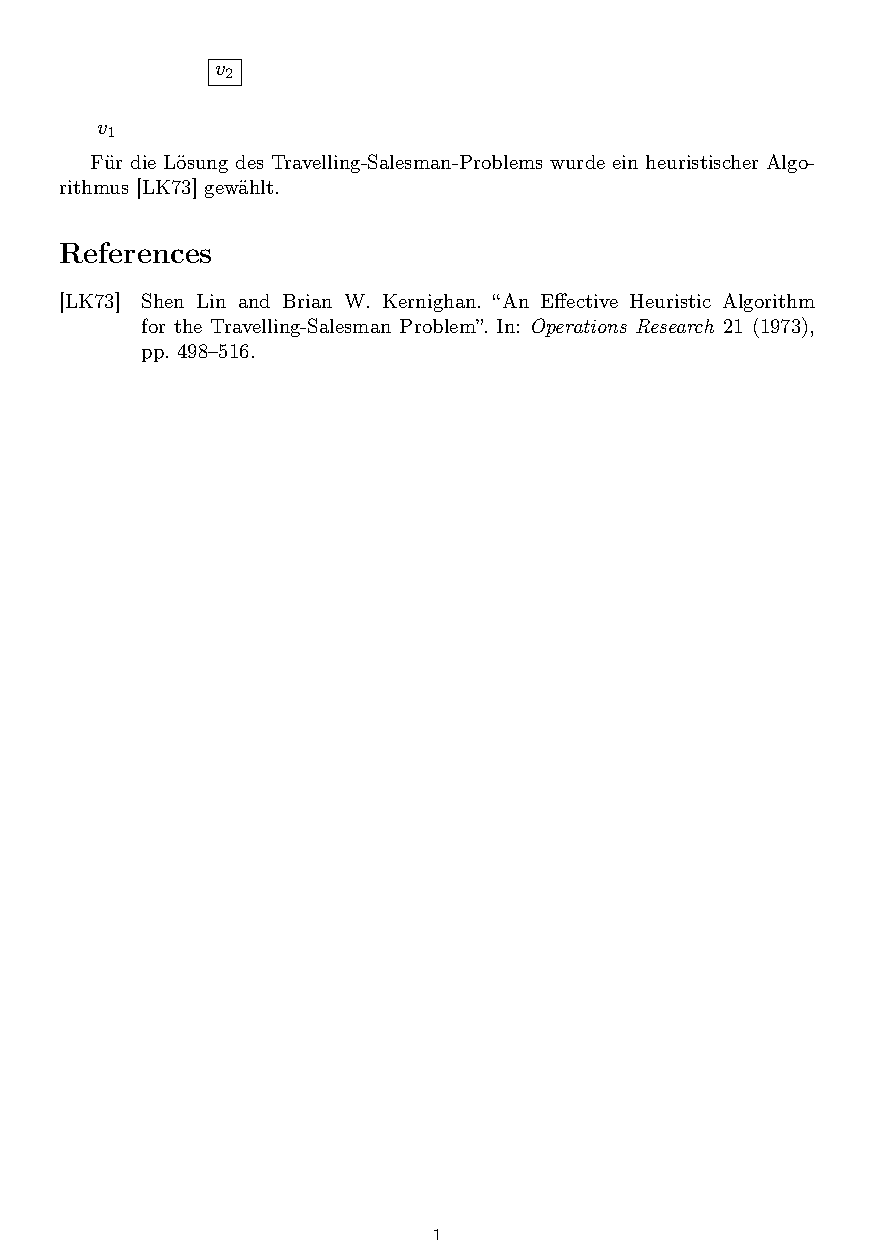
\includegraphics[width=\textwidth]{images/biblatex-example.pdf}
		\end{frame}

	\section{Quellcode}
		\sectionTitleFrame
	
		\subsection{Code-Highlighten}

		%%%%%%%%%%%%%%%%%%%%%%%%%%%%%%%%%%%%%%%%%%%%%%%%%%%%%%%%%%%%%%%%%%%%%%%

		\begin{frame}[containsverbatim]{Mit \texttt{minted}}
			\begin{itemize}
				\item \texttt{minted} arbeitet mit Pygments (python-library).
				\item Benötigt \texttt{-shell-escape} als Parameter von \texttt{pdflatex}.
			\end{itemize}

			\slideheading{\LaTeX-Code:}
			\begin{smalllatexcode}
\usepackage{minted}
% ...
\begin{minted}{java}
class MeineKlasse{
	private int meineVariable; // Deklaration

	public void meineMethode(){
		meineVariable = 42; // Initialisierung
	}
}
\end{minted}
			\end{smalllatexcode}
		\end{frame}

		%%%%%%%%%%%%%%%%%%%%%%%%%%%%%%%%%%%%%%%%%%%%%%%%%%%%%%%%%%%%%%%%%%%%%%%

		\begin{frame}[containsverbatim]{Mit \texttt{minted}}
			\slideheading{Ergebnis:}
			\begin{minted}{java}
class MeineKlasse{
	private int meineVariable; // Deklaration

	public void meineMethode(){
		meineVariable = 42; // Initialisierung
	}
}
			\end{minted}
		\end{frame}

		%%%%%%%%%%%%%%%%%%%%%%%%%%%%%%%%%%%%%%%%%%%%%%%%%%%%%%%%%%%%%%%%%%%%%%%

		\begin{frame}[containsverbatim]{Mit \texttt{lstlisting}}
			\slideheading{\LaTeX-Code:}
			\begin{smallerlatexcode}
\usepackage{listings}
\lstset{...} % Style-Einstellungen
% ...
\begin{lstlisting}[caption=Deklaration und Initialisierung von Variablen]
class MeineKlasse{
	private int meineVariable; // Deklaration

	public void meineMethode(){
		meineVariable = 42; // Initialisierung
	}
}
\end{lstlisting}
			\end{smallerlatexcode}
		\end{frame}

		%%%%%%%%%%%%%%%%%%%%%%%%%%%%%%%%%%%%%%%%%%%%%%%%%%%%%%%%%%%%%%%%%%%%%%%

		\begin{frame}[containsverbatim]{Mit \texttt{lstlisting}}
			\slideheading{Ergebnis:}
			\begin{lstlisting}[caption=Deklaration und Initialisierung von Variablen]
class MeineKlasse{
	private int meineVariable; // Deklaration

	public void meineMethode(){
		meineVariable = 42; // Initialisierung
	}
}
			\end{lstlisting}
		\end{frame}

		%%%%%%%%%%%%%%%%%%%%%%%%%%%%%%%%%%%%%%%%%%%%%%%%%%%%%%%%%%%%%%%%%%%%%%%
		
		\begin{frame}[containsverbatim]{Mit \texttt{verbatim}}
			\slideheading{\LaTeX-Code:}
			\begin{smallerlatexcode}
\begin{verbatim}
~$ cat .ssh/config
Host fbi
  User 7nachnam
  ForwardX11 yes
  HostName rzssh1.informatik.uni-hamburg.de
  DynamicForward 7777
  #LocalForward 6631 linuxprint.informatik.uni-hamburg.de:631
\end{verbatim}
			\end{smallerlatexcode}
		\end{frame}

		%%%%%%%%%%%%%%%%%%%%%%%%%%%%%%%%%%%%%%%%%%%%%%%%%%%%%%%%%%%%%%%%%%%%%%%

		\begin{frame}[containsverbatim]{Mit \texttt{verbatim}}
			\slideheading{Ergebnis:}
{
\small
			\begin{verbatim}
~$ cat .ssh/config
Host fbi
  User 7nachnam
  ForwardX11 yes
  HostName rzssh1.informatik.uni-hamburg.de
  DynamicForward 7777
  #LocalForward 6631 linuxprint.informatik.uni-hamburg.de:631			
			\end{verbatim}
}

		\end{frame}		

		%%%%%%%%%%%%%%%%%%%%%%%%%%%%%%%%%%%%%%%%%%%%%%%%%%%%%%%%%%%%%%%%%%%%%%%
		
		\begin{frame}[containsverbatim]{Mit \texttt{algorithmic} (Pseudocode)}
			\slideheading{\LaTeX-Code:}
			\begin{smalllatexcode}
\begin{algorithmic}
    \IF{some condition is true}
        \STATE do some processing
    \ELSIF{some other condition is true}
        \STATE do some different processing
    \ENDIF
\end{algorithmic}
			\end{smalllatexcode}
			\slideheading{Ergebnis:}

\begin{algorithmic}
    \IF{some condition is true}
        \STATE do some processing
    \ELSIF{some other condition is true}
        \STATE do some different processing
    \ENDIF
\end{algorithmic}

		\end{frame}

		%%%%%%%%%%%%%%%%%%%%%%%%%%%%%%%%%%%%%%%%%%%%%%%%%%%%%%%%%%%%%%%%%%%%%%%

	\section{\LaTeX{} erweitern}
		\sectionTitleFrame
	
		\subsection{Makros \& Umgebungen}
		
		\begin{frame}[containsverbatim]{Eigene Befehle}
			\slideheading{\LaTeX-Code:}
			\begin{latexcode}
% TeX-style
\def\heute{Heute ist der \today.}
% LaTeX-style (besser)
\newcommand{\heute}{Heute ist der \today.}
\newcommand{\TikZ}{Ti\textit{k}Z}
% Verwendung
\heute
\TikZ
			\end{latexcode}
			\slideheading{Ergebnis:}
			Heute ist der \today.\\
			\TikZ
		\end{frame}

		%%%%%%%%%%%%%%%%%%%%%%%%%%%%%%%%%%%%%%%%%%%%%%%%%%%%%%%%%%%%%%%%%%%%%%%

		\begin{frame}[containsverbatim]{Eigene Befehle -- Parameter}
			\slideheading{\LaTeX-Code:}
			\begin{latexcode}
% LaTeX-style
\newcommand{\bus}[4]{Ein Bus der Linie #1 Richtung
                    #2 fährt von der Haltestelle
                    #3 um #4 ab.}
% Verwendung
\bus{181}{Sternschanze}{Informatikum}{13:37}
			\end{latexcode}
			\slideheading{Ergebnis:}
			\bus{181}{Sternschanze}{Informatikum}{13:37}
		\end{frame}
		
		%%%%%%%%%%%%%%%%%%%%%%%%%%%%%%%%%%%%%%%%%%%%%%%%%%%%%%%%%%%%%%%%%%%%%%%
		
		\begin{frame}[containsverbatim]{Eigene Befehle -- Optionale Parameter}
		\slideheading{\LaTeX-Code:}
		\begin{latexcode}
			% LaTeX-style
			\newcommand{\bus}[2][181]{Linie #1 Richtung #2.}
			% Verwendung
			\bus{Sternschanze}
			\bus[22]{Blankenese}
		\end{latexcode}
		\slideheading{Ergebnis:}\\
		\vspace{0.2cm}
		Linie 181 Richtung Sternschanze.
		Linie 22 Richtung Blankenese.
		\end{frame}

		%%%%%%%%%%%%%%%%%%%%%%%%%%%%%%%%%%%%%%%%%%%%%%%%%%%%%%%%%%%%%%%%%%%%%%%

		\begin{frame}[containsverbatim]{Eigene Umgebungen}
			\slideheading{\LaTeX-Code:}
			\begin{latexcode}
\newenvironment{textttit}
               {\begingroup\ttfamily\itshape}
               {\endgroup}
% Verwendung
\begin{textttit}
	Dies ist ein Test
\end{textttit}
			\end{latexcode}
			\slideheading{Ergebnis:}
			\texttt{\textit{Dies ist ein Test}}
		\end{frame}
		
		%%%%%%%%%%%%%%%%%%%%%%%%%%%%%%%%%%%%%%%%%%%%%%%%%%%%%%%%%%%%%%%%%%%%%%%

		\subsection{Packages \& Klassen}

		\begin{frame}[containsverbatim]{Eigene Packages}
			\slideheading{\LaTeX-Code (meinpackage.sty):}
			\begin{smallerlatexcode}
\NeedsTeXFormat{LaTeX2e}
\ProvidesPackage{meinpackage}[2000/01/01 Mein Package]

\newcommand{\helloworld}{Hello World!}

\DeclareOption{german}{
  \renewcommand{\helloworld}{Hallo Welt!}
}

\ProcessOptions\relax

\endinput
			\end{smallerlatexcode}
		\end{frame}
		
		%%%%%%%%%%%%%%%%%%%%%%%%%%%%%%%%%%%%%%%%%%%%%%%%%%%%%%%%%%%%%%%%%%%%%%%

		\begin{frame}[containsverbatim]{Eigene Dokumentenklassen}
			\slideheading{\LaTeX-Code (meineklasse.cls):}
			\begin{smalllatexcode}
\NeedsTeXFormat{LaTeX2e}
\ProvidesClass{meineklasse}[2000/01/01 Meine Klasse]

\RequirePackage[utf8]{inputenc}
\RequirePackage[T1]{fontenc}
\RequirePackage[ngerman]{babel}
\RequirePackage{lmodern}

\DeclareOption{sans}{
  \renewcommand*\familydefault{\sfdefault}
}

\ProcessOptions\relax

\LoadClass[a4paper,10pt]{scrartcl}

\endinput
			\end{smalllatexcode}
		\end{frame}
		
		%%%%%%%%%%%%%%%%%%%%%%%%%%%%%%%%%%%%%%%%%%%%%%%%%%%%%%%%%%%%%%%%%%%%%%%

		\begin{frame}[containsverbatim]{Benutzung}
			\begin{columns}[t]
				\column{.6\textwidth}
				\slideheading{\LaTeX-Code:}
				\begin{smallerlatexcode}
\documentclass[sans]{meineklasse}

\usepackage[german]{meinpackage}

\begin{document}
	\helloworld
\end{document}
				\end{smallerlatexcode}
				\column{.4\textwidth}
				\vspace*{10mm}
				\begin{minipage}{\textwidth}
					\begin{center}
						\slideheading{Ergebnis:}
						\\[5mm]
						\textsf{Hallo Welt!}
					\end{center}
				\end{minipage}
			\end{columns}
			\vspace*{5mm}			
			\slideheading{Mehr Infos:}
			\url{http://ctan.mirrors.hoobly.com/macros/latex/doc/clsguide.pdf}
			\\
			\url{https://en.wikibooks.org/wiki/LaTeX/Creating_Packages}	
		\end{frame}
		
		%%%%%%%%%%%%%%%%%%%%%%%%%%%%%%%%%%%%%%%%%%%%%%%%%%%%%%%%%%%%%%%%%%%%%%%

		\begin{frame}[containsverbatim]{Alternative: Include-Dateien}
			\begin{itemize}
				\item \texttt{\textbackslash{}input\{<datei>\}} lädt den Inhalt von \texttt{<datei>} stumpf, als ob er so im Dokument stehen würde.
				\item \texttt{\textbackslash{}include\{<datei>\}} macht eine neue Seite auf und kann nicht geschachtelt werden, legt aber eigene \texttt{aux}-Dateien an und kann somit Seitenzahlen und Querverweise beachten.
			\end{itemize}
	
			\slideheading{\LaTeX-Code (beispiel.inc):}
			\begin{latexcode}
Hallo \LaTeX!
			\end{latexcode}
			\slideheading{\LaTeX-Code (Hauptdokument):}
			\begin{latexcode}
\input{beispiel.inc}
			\end{latexcode}
			\slideheading{Ergebnis:}
			
			Hallo \LaTeX!
		\end{frame}
		
		%%%%%%%%%%%%%%%%%%%%%%%%%%%%%%%%%%%%%%%%%%%%%%%%%%%%%%%%%%%%%%%%%%%%%%%		
		
	\section{Math advanced}
		\sectionTitleFrame
		
		\subsection{Math advanced}
		
		\begin{frame}[containsverbatim]{Mehr tolle Mathe-Tricks}
			\slideheading{\LaTeX-Code:}
			\begin{smalllatexcode}
Große Klammern gehen auch: \(\left( \frac{n^2 + 1}{3} \right)^2\) \\
Aus \(\int_a^b \ \sum_a^b\) wird \(\displaystyle \int\limits_a^b \ \sum_a^b \)
			\end{smalllatexcode}
			\slideheading{Ergebnis:}

Große Klammern gehen auch: \(
\displaystyle \left( \frac{n^2 + 1}{3} \right)^2
\)\\
Aus \(\int_a^b \ \sum_a^b\) wird \(\displaystyle \ \int\limits_a^b \ \sum_a^b  \)



			\slideheading{Anmerkung:} Über \texttt{\textbackslash{}everymath\{\textbackslash{}displaystyle\}} kann jeder Mathe-Modus automatisch im \texttt{displaystyle} sein.

		\end{frame}
		
		%%%%%%%%%%%%%%%%%%%%%%%%%%%%%%%%%%%%%%%%%%%%%%%%%%%%%%%%%%%%%%%%%%%%%%%		

		\begin{frame}[containsverbatim]{Mehr Mathe mit \texttt{mathtools}}
			\slideheading{\LaTeX-Code:}
			\begin{smalllatexcode}
\mathsf{sinc}(x) \coloneqq
\begin{dcases}
	1                 & x = 0 \\
	\frac{\sin(x)}{x} & \text{sonst}
\end{dcases}
			\end{smalllatexcode}
			\vspace{0.3cm}
			\slideheading{Ergebnis:}
			\vspace{0.1cm}\\
			\(
			\mathsf{sinc}(x) \coloneqq
			\begin{dcases}
				1                 & x = 0 \\
				\frac{\sin(x)}{x} & \text{sonst}
			\end{dcases}
			\)
		\end{frame}
		
		%%%%%%%%%%%%%%%%%%%%%%%%%%%%%%%%%%%%%%%%%%%%%%%%%%%%%%%%%%%%%%%%%%%%%%%		
		
		\begin{frame}[containsverbatim]{Mehr Mathe mit \texttt{mathtools}}
			\slideheading{\LaTeX-Code:}
			\begin{smalllatexcode}
\underbrace{\exp(i x)}_{\text{Hier wird es hässlich}}
=
\cos(x) + \underbracket{i \sin(x)}_{\mathclap{\text{Hier wird es hübsch}}}
			\end{smalllatexcode}
			\vspace{0.3cm}
			\slideheading{Ergebnis:}
			\vspace{0.1cm}\\
			\(
				\underbrace{\exp(i x)}_{\text{Hier wird es hässlich}} = \cos(x) + \underbracket{i \sin(x)}_{\mathclap{\text{Hier wird es hübsch}}}
			\)
		\end{frame}
		
		%%%%%%%%%%%%%%%%%%%%%%%%%%%%%%%%%%%%%%%%%%%%%%%%%%%%%%%%%%%%%%%%%%%%%%%		

		\begin{frame}[containsverbatim]{SI-Einheiten mit \texttt{siunitx}}
			\slideheading{\LaTeX-Code:}
			\begin{latexcode}
\sisetup{...} % Einstellungen für siunitx
Wissenschaftliche Notation: \(n = \num{1.1e3}\) \\
Einheiten: \(\si{\J} = \si{\kg\m\squared\per\s\squared}\) \\
Kombiniert: \(\SI{50}{\percent} c = \SI{1.5e8}{\m\per\s}\) \\
Intervalle: \(\SIrange{1.3e5}{3.6e6}{\kg\m\per\s}\)
			\end{latexcode}
			\slideheading{Ergebnis:}

\sisetup{%
  locale = DE,
  per-mode = fraction,
  range-phrase = \text{--},
  range-units = single
}

Wissenschaftliche Notation: \(n = \num{1.1e3}\) \\
Einheiten: \(\si{\J} = \si{\kg\m\squared\per\s\squared}\) \\
Kombiniert: \(\SI{50}{\percent} c = \SI{1.5e8}{\m\per\s}\) \\
Intervalle: \(\SIrange{1.3e5}{3.6e6}{\kg\m\per\s}\)

		\end{frame}
		
		%%%%%%%%%%%%%%%%%%%%%%%%%%%%%%%%%%%%%%%%%%%%%%%%%%%%%%%%%%%%%%%%%%%%%%%		

		\begin{frame}[containsverbatim]{Noch mehr Mathe mit \texttt{physics}}
			\slideheading{\LaTeX-Code:}
			\begin{latexcode}
Beträge und Normen:
\(\norm{\vec{x}} = \sum_{k=1}^n \abs{x_k}^2 \) \\
Landau-Notation: \(\order{n \cdot \log(n)} \) \\
Differentiale: \(\int f(x) \dd{x};
\quad \dv{f}{x}; \quad \pdv[2]{f}{x}\)
			\end{latexcode}
			\slideheading{Ergebnis:}

Beträge und Normen: \(\displaystyle \norm{\vec{x}} = \sum_{k=1}^n \abs{x_k}^2 \) \\
Landau-Notation: \(\displaystyle \order{n \cdot \log(n)} \) \\
Differentiale: \(\displaystyle \int f(x) \dd{x}; \quad \dv{f}{x}; \quad \pdv[2]{f}{x}\) \\

		\end{frame}		
		

		%%%%%%%%%%%%%%%%%%%%%%%%%%%%%%%%%%%%%%%%%%%%%%%%%%%%%%%%%%%%%%%%%%%%%%%

%		\section{HA-Tipps}
%
%		\begin{frame}[containsverbatim]{\LaTeX{}-Beamer}
%			\begin{center}
%				Und jetzt ein paar Tipps für Hausaufgaben/-arbeiten
%			\end{center}
%		\end{frame}

		%%%%%%%%%%%%%%%%%%%%%%%%%%%%%%%%%%%%%%%%%%%%%%%%%%%%%%%%%%%%%%%%%%%%%%%

	\section{\protect\TikZ}
		\sectionTitleFrame
		
		\subsection{\protect\TikZ}

		\begin{frame}[containsverbatim]{\TikZ}
			\begin{itemize}
				\item \textbf{T}ikZ \textbf{i}st \textbf{k}ein \textbf{Z}eichenprogramm.
				\item Abbildungen werden mit TikZ beschrieben und durch PGF gerendert.
				\item Sehr umfangreiches Paket (Dokumentation: $>$1000 Seiten) mit vielen Möglichkeiten.
				\item Direkte Unterstützung für Petrinetze \&\newline Automaten ;-)
			\end{itemize}


			\vspace{-1.25cm}
			\hspace{8.5cm}
			\begin{tikzpicture}
				\draw[thick,rounded corners=8pt]
				(0,0) -- (0,2) -- (1,3.25) -- (2,2) --
				(2,0) -- (0,2) -- (2,2) -- (0,0) -- (2,0);
			\end{tikzpicture}
		\end{frame}

		%%%%%%%%%%%%%%%%%%%%%%%%%%%%%%%%%%%%%%%%%%%%%%%%%%%%%%%%%%%%%%%%%%%%%%%

		\subsection{Grundlagen}
		
		\begin{frame}[containsverbatim]{\TikZ}
			\begin{columns}[t]
				\column{0.7\textwidth}
				\slideheading{\LaTeX{}-Code:}
				\begin{latexcode}
\begin{tikzpicture}
	\node (v1) at (0,0) {$v_1$};
	
	\coordinate (c) at (2, 1);
	\node[draw,rectangle] (v2)
	    at (c) {$v_2$};
\end{tikzpicture}
				\end{latexcode}
				
				\column{0.3\textwidth}
				\hspace{3mm}
				\slideheading{Ergebnis:}\\
				\hspace{3mm}
				\vspace{0.2cm}
				\begin{tikzpicture}
					\node (v1) at (0,0) {$v_1$};
					
					\coordinate (c) at (2, 1);
					\node[draw,rectangle] (v2) at (c) {$v_2$};
				\end{tikzpicture}
			\end{columns}
		\end{frame}
		
		%%%%%%%%%%%%%%%%%%%%%%%%%%%%%%%%%%%%%%%%%%%%%%%%%%%%%%%%%%%%%%%%%%%%%%%
		
		\subsection{Grundlagen}
		
		\begin{frame}[containsverbatim]{\TikZ}
			\begin{columns}[t]
				\column{0.7\textwidth}
				\slideheading{\LaTeX{}-Code:}
				\begin{latexcode}
\begin{tikzpicture}
	\node (v) at (3,1) {$v$};
	
	\draw (0,0) -- (2,0) --
          (2,1) -- (v);
\end{tikzpicture}
				\end{latexcode}
				
				\column{0.3\textwidth}
				\hspace{3mm}
				\slideheading{Ergebnis:}\\
				\hspace{3mm}
				\vspace{0.2cm}
				\begin{tikzpicture}
					\node (v) at (3,1) {$v$};
					
					\draw (0,0) -- (2,0) --
					      (2,1) -- (v);
				\end{tikzpicture}
			\end{columns}
		\end{frame}
		
		%%%%%%%%%%%%%%%%%%%%%%%%%%%%%%%%%%%%%%%%%%%%%%%%%%%%%%%%%%%%%%%%%%%%%%%

		\begin{frame}[containsverbatim]{\TikZ}
			\begin{columns}[t]
				\column{0.7\textwidth}
				\slideheading{\LaTeX{}-Code:}
				\begin{latexcode}
\begin{tikzpicture}
	\draw[thick,rounded corners=8pt]
		(0,0) -- (0,2) -- (1,3.25) --
		(2,2) -- (2,0) -- (0,2) --
		(2,2) -- (0,0) -- (2,0);
\end{tikzpicture}
				\end{latexcode}

				\column{0.3\textwidth}
				\hspace{3mm}
				\slideheading{Ergebnis:}
				\hspace{3mm}
				\begin{tikzpicture}
					\draw[thick,rounded corners=8pt]
					(0,0) -- (0,2) -- (1,3.25) -- (2,2) --
					(2,0) -- (0,2) -- (2,2) -- (0,0) -- (2,0);
				\end{tikzpicture}
			\end{columns}
		\end{frame}

		%%%%%%%%%%%%%%%%%%%%%%%%%%%%%%%%%%%%%%%%%%%%%%%%%%%%%%%%%%%%%%%%%%%%%%%

		\begin{frame}[containsverbatim]{Nodes und Lines}
			\slideheading{\TikZ-Code:}
			\begin{latexcode}
\begin{tikzpicture}
	\node[red]       (s) at (0, 0) {S};
	\node[fill=gray] (t) at (3, 0) {T};

	\draw[thick, ->]     (s)     -- (1, -1);
	\draw[thick, dotted]
		(1, -1) to [bend right = 45] (2, -1);
	\draw[thick,->]      (2, -1) -- (t);
\end{tikzpicture}
			\end{latexcode}
		\end{frame}

		%%%%%%%%%%%%%%%%%%%%%%%%%%%%%%%%%%%%%%%%%%%%%%%%%%%%%%%%%%%%%%%%%%%%%%%

		\begin{frame}[containsverbatim]{Nodes und Lines}
			\slideheading{Ergebnis:}\\
			\vspace{0.5cm}
			\begin{center}
				\begin{tikzpicture}
					\node[red] (s) at (0, 0) {S};
					\node[fill=gray] (t) at (3, 0) {T};

					\draw[thick, ->]     (s)     -- (1, -1);
					\draw[thick, dotted]
						(1, -1) to [bend right = 45] (2, -1);
					\draw[thick,->]      (2, -1) -- (t);
				\end{tikzpicture}
			\end{center}
		\end{frame}

%		%%%%%%%%%%%%%%%%%%%%%%%%%%%%%%%%%%%%%%%%%%%%%%%%%%%%%%%%%%%%%%%%%%%%%%%
%
%		\begin{frame}[containsverbatim]{Hobby-Kurven}
%			\begin{itemize}
%				\item Hobby-Kurven mittels \texttt{hobby}-Paket
%			\end{itemize}
%			\slideheading{\TikZ-Code:}
%			\begin{smalllatexcode}
%\begin{tikzpicture}
%	\node[red]       (s) at (0, 0) {S};
%	\node[fill=gray] (t) at (3, 0) {T};
%
%	\draw[thick, ->]     (s)     -- (1, -1);
%	\draw[thick, ->, dotted]
%		(1, -1)
%		to[curve through={(1.5, -1.1) .. (1.5,-0.75) .. (1.5, -1.1)}]
%		(2, -1);
%	\draw[thick, ->]      (2, -1) -- (t);
%\end{tikzpicture}
%			\end{smalllatexcode}
%		\end{frame}
%
%		%%%%%%%%%%%%%%%%%%%%%%%%%%%%%%%%%%%%%%%%%%%%%%%%%%%%%%%%%%%%%%%%%%%%%%%
%
%		\begin{frame}[containsverbatim]{Hobby-Kurven}
%			\begin{center}
%				\slideheading{Ergebnis:}
%				\vspace{0.5cm}
%				\begin{tikzpicture}
%					\node[red]       (s) at (0, 0) {S};
%					\node[fill=gray] (t) at (3, 0) {T};
%
%					\draw[thick, ->]     (s)     -- (1, -1);
%					\draw[thick, ->, dotted]
% 						(1, -1)
% 						to[curve through={(1.5, -1.1) .. (1.5,-0.75) .. (1.5, -1.1)}]
% 						(2, -1);
%					\draw[thick, ->]      (2, -1) -- (t);
%				\end{tikzpicture}
%			\end{center}
%		\end{frame}

		%%%%%%%%%%%%%%%%%%%%%%%%%%%%%%%%%%%%%%%%%%%%%%%%%%%%%%%%%%%%%%%%%%%%%%%

		\begin{frame}[containsverbatim]{Styles für gesamtes \TikZ picture}
			\slideheading{\TikZ-Code:}
			\begin{smalllatexcode}
\begin{tikzpicture}
	[
		->, thick,
		knoten/.style={shape=rectangle,draw=black,rounded corners}
	]
	\node[knoten] (s) at (0, 0) {S};
	\node[knoten] (t) at (3, 0) {T};
	\draw[->] (s) -- (t);
\end{tikzpicture}
			\end{smalllatexcode}
			\vspace{0.2cm}
			\slideheading{Ergebnis:}\\
			\begin{center}
				\begin{tikzpicture}
					[
						->, thick,
						knoten/.style={shape=rectangle,draw=black,rounded corners}
					]
					\node[knoten] (s) at (0, 0) {S};
					\node[knoten] (t) at (3, 0) {T};
					\draw[->] (s) -- (t);
				\end{tikzpicture}
			\end{center}
		\end{frame}

		%%%%%%%%%%%%%%%%%%%%%%%%%%%%%%%%%%%%%%%%%%%%%%%%%%%%%%%%%%%%%%%%%%%%%%%

		\subsection{Automaten}

		\begin{frame}[containsverbatim]{Einführung}
			\begin{itemize}
				\item Automaten (state machines) per \texttt{automata}-Paket
				\item Für Positionierung \texttt{positioning}-Paket
				\item Und für Pfeile \texttt{arrows}-Paket
			\end{itemize}
			Mehr Informationen über Automaten, Pfeile, Positionierung, Optionen, etc. gibt es unter \href{http://hauke-stieler.de/public/tikz-for-state-machines.pdf}{hauke-stieler.de/public/tikz-for-state-machines.pdf}\\
			{\tiny(im selben Ordner ist auch die entsprechende \texttt{*.tex} Datei)}
		\end{frame}

		%%%%%%%%%%%%%%%%%%%%%%%%%%%%%%%%%%%%%%%%%%%%%%%%%%%%%%%%%%%%%%%%%%%%%%%

		\begin{frame}[containsverbatim]{Zustände}
			\slideheading{\TikZ-Code:}
			\begin{smallerlatexcode}
\usetikzlibrary{
	automata,
	arrows}
% ...
\begin{tikzpicture}[->,
	>=stealth',
	semithick]

	\node[state,initial]   (0)              {$z_0$};
	\node[state]           (1) [right of=0] {$z_1$};
	\node[state,accepting] (2) [right of=1] {$z_2$};
\end{tikzpicture}
			\end{smallerlatexcode}
		\end{frame}

		%%%%%%%%%%%%%%%%%%%%%%%%%%%%%%%%%%%%%%%%%%%%%%%%%%%%%%%%%%%%%%%%%%%%%%%

		\begin{frame}[containsverbatim]{Zustände}
			\slideheading{Ergebnis:}\\
			\vspace{0.5cm}
			\begin{center}
				\begin{tikzpicture}[->,
					>=stealth',
					semithick]

					\node[state,initial]   (0)              {$z_0$};
					\node[state]           (1) [right of=0] {$z_1$};
					\node[state,accepting] (2) [right of=1] {$z_2$};
				\end{tikzpicture}
			\end{center}
		\end{frame}

		%%%%%%%%%%%%%%%%%%%%%%%%%%%%%%%%%%%%%%%%%%%%%%%%%%%%%%%%%%%%%%%%%%%%%%%

		\begin{frame}[containsverbatim]{Positionierung}
			\slideheading{\TikZ-Code:}
			\begin{smalllatexcode}
\usetikzlibrary{
	automata,
	arrows,
	positioning}
% ...
\begin{tikzpicture}[->,
	>=stealth',
	semithick,
	node distance=2cm]

	\node [state] (a)                                {$a$};
	\node [state] (b) [above right=1cm and 2cm of a] {$b$};
	\node [state] (c) [below right of = a]           {$c$};
\end{tikzpicture}
			\end{smalllatexcode}
		\end{frame}

		%%%%%%%%%%%%%%%%%%%%%%%%%%%%%%%%%%%%%%%%%%%%%%%%%%%%%%%%%%%%%%%%%%%%%%%

		\begin{frame}[containsverbatim]{Positionierung}
			\slideheading{Ergebnis:}\\
			\vspace{0.5cm}
			\begin{center}
				\begin{tikzpicture}[->,
					>=stealth',
					semithick,
					node distance=2cm]

					\node [state] (a)                                {$a$};
					\node [state] (b) [above right=1cm and 2cm of a] {$b$};
					\node [state] (c) [below right of = a]           {$c$};
				\end{tikzpicture}
			\end{center}
		\end{frame}

		%%%%%%%%%%%%%%%%%%%%%%%%%%%%%%%%%%%%%%%%%%%%%%%%%%%%%%%%%%%%%%%%%%%%%%%

		\begin{frame}[containsverbatim]{Genauere Positionierung}
			\begin{columns}[t]
				\column{0.775\textwidth}
				\slideheading{\LaTeX{}-Code:}
				\begin{smalllatexcode}
\usetikzlibrary{calc}
% ...
\begin{tikzpicture}
	\node [state] (a)                                {$a$};
	\node [state] (b) [below right=1cm and 2cm of a] {$b$};
	\node [state] (c) [at=(a|-b)]                    {$c$};
	\node [state] (d) [at=(b|-a)]                    {$d$};
	\node [state] (e) [at=($(a)!1/2!(d)$)]           {$e$};
	\node [state] (f) [at=($(a)!2!(c)$)]             {$f$};
\end{tikzpicture}
				\end{smalllatexcode}

				\column{0.225\textwidth}
				\hspace{3mm}
				\slideheading{Ergebnis:}\\
				\hspace{3mm}
				\scalebox{0.75}{
					\begin{tikzpicture}
						\node [state] (a)                                {$a$};
						\node [state] (b) [below right=1cm and 2cm of a] {$b$};
						\node [state] (c) [at=(a|-b)]					{$c$};
						\node [state] (d) [at=(b|-a)]					{$d$};
						\node [state] (e) [at=($(a)!1/2!(d)$)] 			{$e$};
						\node [state] (f) [at=($(a)!2!(c)$)]				{$f$};
					\end{tikzpicture}
				}
			\end{columns}
		\end{frame}

		%%%%%%%%%%%%%%%%%%%%%%%%%%%%%%%%%%%%%%%%%%%%%%%%%%%%%%%%%%%%%%%%%%%%%%%

		\begin{frame}[containsverbatim]{Pfeile}
			\slideheading{\TikZ-Code:}
			\begin{smalllatexcode}
\begin{tikzpicture}[->,
	>=stealth',
	semithick,
	node distance=2cm]

	\node [state,initial]   (a)            {$a$};
	\node [state]           (b)
		[above right=1cm and 2cm of a]     {$b$};
	\node [state,accepting] (c)
		[below right = 1cm and 1.5cm of a] {$c$};

	\path (a) edge node {0} (b)
	          edge node {1} (c)
	      (c) edge node {2} (b);
\end{tikzpicture}
			\end{smalllatexcode}
		\end{frame}

		%%%%%%%%%%%%%%%%%%%%%%%%%%%%%%%%%%%%%%%%%%%%%%%%%%%%%%%%%%%%%%%%%%%%%%%

		\begin{frame}[containsverbatim]{Pfeile}
			\slideheading{Ergebnis:}\\
			\vspace{0.5cm}
			\begin{center}
				\begin{tikzpicture}[->,
					>=stealth',
					semithick,
					node distance=2cm]

					\node [state,initial]   (a)            {$a$};
					\node [state]           (b)
						[above right=1cm and 2cm of a]     {$b$};
					\node [state,accepting] (c)
						[below right = 1cm and 1.5cm of a] {$c$};

					\path (a) edge node {0} (b)
					          edge node {1} (c)
					      (c) edge node {2} (b);
				\end{tikzpicture}
			\end{center}
		\end{frame}

		%%%%%%%%%%%%%%%%%%%%%%%%%%%%%%%%%%%%%%%%%%%%%%%%%%%%%%%%%%%%%%%%%%%%%%%

		\begin{frame}[containsverbatim]{Pfeile}
			\slideheading{\TikZ-Code:}
			\begin{smalllatexcode}
\begin{tikzpicture}[->,
	>=stealth',
	semithick,
	node distance=2cm]

	\node [state,initial]   (a)            {$a$};
	\node [state]           (b)
		[above right=1cm and 2cm of a]     {$b$};
	\node [state,accepting] (c)
		[below right = 1cm and 1.5cm of a] {$c$};

	\path (a) edge[above] node {0} (b)
	          edge[below] node {1} (c)
	      (c) edge[right] node {2} (b);
\end{tikzpicture}
			\end{smalllatexcode}
		\end{frame}

		%%%%%%%%%%%%%%%%%%%%%%%%%%%%%%%%%%%%%%%%%%%%%%%%%%%%%%%%%%%%%%%%%%%%%%%

		\begin{frame}[containsverbatim]{Pfeile}
			\slideheading{Ergebnis:}\\
			\vspace{0.5cm}
			\begin{center}
				\begin{tikzpicture}[->,
					>=stealth',
					semithick,
					node distance=2cm]

					\node [state,initial]   (a)            {$a$};
					\node [state]           (b)
						[above right=1cm and 2cm of a]     {$b$};
					\node [state,accepting] (c)
						[below right = 1cm and 1.5cm of a] {$c$};

					\path (a) edge[above] node {0} (b)
					          edge[below] node {1} (c)
					      (c) edge[right] node {2} (b);
				\end{tikzpicture}
			\end{center}
		\end{frame}

		%%%%%%%%%%%%%%%%%%%%%%%%%%%%%%%%%%%%%%%%%%%%%%%%%%%%%%%%%%%%%%%%%%%%%%%

		\begin{frame}[containsverbatim]{Pfeile}
			\slideheading{\TikZ-Code:}
			\begin{smalllatexcode}
\begin{tikzpicture}[->,>=stealth',
	shorten >=5pt,
	node distance=2.5cm,
	semithick]

	\node[initial,state]   (R)              {$z_r$};
	\node[state]           (S) [right of=R] {$z_s$};
	\node[state,accepting] (E) [right of=S] {$z_e$};

	\path   (R) edge [loop,above]       node {0}   (R)
				edge [below]            node {1}   (S)
		    (S) edge [loop,above]       node {0,1} (S)
				edge [below]            node {1}   (E)
		    (E) edge [bend left,below]  node {0}   (R)
				edge [loop,above]       node {0,1} (E);
\end{tikzpicture}
			\end{smalllatexcode}
		\end{frame}

		%%%%%%%%%%%%%%%%%%%%%%%%%%%%%%%%%%%%%%%%%%%%%%%%%%%%%%%%%%%%%%%%%%%%%%%

		\begin{frame}[containsverbatim]{Pfeile}
			\slideheading{Ergebnis:}\\
			\vspace{0.5cm}
			\begin{center}
				\begin{tikzpicture}[->,>=stealth',
					shorten >=5pt,
					node distance=2.5cm,
					semithick]

					\node[initial,state]   (R)              {$z_r$};
					\node[state]           (S) [right of=R] {$z_s$};
					\node[state,accepting] (E) [right of=S] {$z_e$};

					\path 	(R)	edge [loop,above]       node {0} (R)
								edge [below]            node {1} (S)
							(S)	edge [loop,above]       node {0,1} (S)
								edge [below]            node {1} (E)
							(E)	edge [bend left,below]  node {0} (R)
								edge [loop,above]       node {0,1} (E);
				\end{tikzpicture}
			\end{center}
		\end{frame}

		%%%%%%%%%%%%%%%%%%%%%%%%%%%%%%%%%%%%%%%%%%%%%%%%%%%%%%%%%%%%%%%%%%%%%%%

		\subsection{Funktionen Zeichnen}

		\begin{frame}[containsverbatim]{\TikZ}
			\begin{smalllatexcode}
\usepackage{pgf}
% ...
\begin{tikzpicture}[>=latex,semithick,font=\scriptsize,scale=0.75]
	\draw[very thin,color=lightgray] (-3.2,-1.2) grid (3.2,4.2);
	\draw[->] (-3.2,0) -- (3.4,0) node[right] {$x$};
	\draw[->] (0,-1.2) -- (0,4.4) node[above] {$y$};

	\foreach \x/\xtext in {-3/-3, -2/-2, -1/-1, 1/1, 2/2, 3/3}
	\draw[shift={(\x,0)}] (0pt,2pt) -- (0pt,-2pt) node[below] {$\xtext$};

	\foreach \y/\ytext in {-1/-1, 1/1, 2/2, 3/3, 4/4}
	\draw[shift={(0,\y)}] (2pt,0pt) -- (-2pt,0pt) node[left] {$\ytext$};

	\draw[thin,domain=-2.075:2.075,smooth,variable=\x,black]
		plot ({\x},{\x*\x});
	\draw[thin] node[inner sep=1mm, fill=white, draw=lightgray]
	    at (2.25,3) {$f(x)=x^2$};
\end{tikzpicture}
			\end{smalllatexcode}
		\end{frame}

		%%%%%%%%%%%%%%%%%%%%%%%%%%%%%%%%%%%%%%%%%%%%%%%%%%%%%%%%%%%%%%%%%%%%%%%

		\begin{frame}{\TikZ}
%			\begin{center}
				\slideheading{Ergebnis:}
				
				\begin{tikzpicture}[>=latex,semithick,font=\scriptsize,scale=0.75]
					\draw[very thin,color=lightgray] (-3.2,-1.2) grid (3.2,4.2);

					\draw[->] (-3.2,0) -- (3.4,0) node[right] {$x$};
					\draw[->] (0,-1.2) -- (0,4.4) node[above] {$y$};

					\foreach \x/\xtext in {-3/-3, -2/-2, -1/-1, 1/1, 2/2, 3/3}
					\draw[shift={(\x,0)}] (0pt,2pt) -- (0pt,-2pt) node[below] {$\xtext$};

					\foreach \y/\ytext in {-1/-1, 1/1, 2/2, 3/3, 4/4}
					\draw[shift={(0,\y)}] (2pt,0pt) -- (-2pt,0pt) node[left] {$\ytext$};

					\draw[thin,domain=-2.075:2.075,smooth,variable=\x,black]
						plot ({\x},{\x*\x});
					\draw[thin] node[inner sep=1mm,
									fill=white,
									draw=lightgray] at (2.25,3) {$f(x)=x^2$};
				\end{tikzpicture}

				\slideheading{Alternative:}
				Gnuplot lässt sich vielfältig mit \LaTeX{} kombinieren
%			\end{center}
		\end{frame}

%		%%%%%%%%%%%%%%%%%%%%%%%%%%%%%%%%%%%%%%%%%%%%%%%%%%%%%%%%%%%%%%%%%%%%%%%
%
%		\subsection{\protect\TikZ{} an die Grenzen getrieben}
%
%		\begin{frame}[containsverbatim]{Banyan-Netz (3 Stufen)}
%			\begin{center}
%				\vspace{-1.5cm}
%				\hspace{-1.5cm}
%				\begin{tikzpicture}
%				[
%					scale = 0.75,
%					transform shape
%				]
%					\banyan{3}
%				\end{tikzpicture}
%			\end{center}
%		\end{frame}
%
%		%%%%%%%%%%%%%%%%%%%%%%%%%%%%%%%%%%%%%%%%%%%%%%%%%%%%%%%%%%%%%%%%%%%%%%%
%
%		\begin{frame}[containsverbatim]{Banyan-Netz (5 Stufen)}
%			\begin{center}
%				\vspace{-0.5cm}
%				\hspace{-1cm}
%				\begin{tikzpicture}
%				[
%					scale = 0.19,
%					transform shape
%				]
%					\banyan{5}
%				\end{tikzpicture}
%			\end{center}
%		\end{frame}
%
%		%%%%%%%%%%%%%%%%%%%%%%%%%%%%%%%%%%%%%%%%%%%%%%%%%%%%%%%%%%%%%%%%%%%%%%%
%
%		\begin{frame}[containsverbatim]{5-dimensionaler Hyperwürfel}
%			\begin{center}
%				\begin{tikzpicture}
%				[
%					scale = 0.5,
%					transform shape,
%				]
%					\hypercube
%				\end{tikzpicture}
%			\end{center}
%		\end{frame}
%
%		%%%%%%%%%%%%%%%%%%%%%%%%%%%%%%%%%%%%%%%%%%%%%%%%%%%%%%%%%%%%%%%%%%%%%%%
%
%		\begin{frame}[containsverbatim]{}
%			\begin{center}
%				... mehrere kaputte Kaffeemaschinen später ...
%			\end{center}
%		\end{frame}
%
%		%%%%%%%%%%%%%%%%%%%%%%%%%%%%%%%%%%%%%%%%%%%%%%%%%%%%%%%%%%%%%%%%%%%%%%%
%
%		\begin{frame}[containsverbatim]{\TikZ{} at its best}
%			\begin{center}
%				\begin{tikzpicture}[scale=0.6,
%				        %Option for nice arrows%
%				        >=latex,%
%				        inner sep=0pt,%
%				        outer sep=2pt,%
%				        mark coordinate/.style={outer sep=0pt,
%				            minimum size=3pt, fill=black,circle}%
%				    ]
%				    %% some definitions
%				    \def\R{0.5}       % sphere radius
%				    \def\angEl{30}    % elevation angle
%				    \def\angAz{-140}  % azimuth angle
%				    \def\angPhi{-105} % longitude of point
%				    \def\angBeta{55}  % latitude of point
%				    \def\angGam{-190} % longitude of point
%				    %% working planes
%				    \pgfmathsetmacro\H{\R*cos(\angEl)}          % Distance to north pole
%				    \LongitudePlane[xzplane]{\angEl}{\angAz}    % x-axis plane
%				    %
%				    \coordinate (O) at (0,0);
%				    %
%				    \begin{scope}[rotate around={-11.1:(0,0)},
%				        field line/.style={color=red, smooth,
%				            variable=\t, samples at={0,-5,-10,...,-360}}
%				    ]
%				        \clip[rotate around={11.1:(0,0)}] (-7,5) rectangle (7,-5);
%
%				        % Computes a point on a field line given r and t
%				        \newcommand{\fieldlinecurve}[2]{%
%				            {(pow(#1,2))*(3*cos(#2)+cos(3*#2))}, {(pow(#1,2))*(sin(#2)+sin(3*#2))}%
%				        }
%
%				        % Longitudinal plnaes
%				        \foreach \u in {0,-40,...,-160}{
%				            \LongitudePlane[{{\u}zplane}]{\angEl}{\u}
%				            \foreach \r in {0.25,0.5,...,2.25} {
%				                \draw[{{\u}zplane}, field line]
%				                plot (\fieldlinecurve{\r}{\t});
%				            }
%				        }
%				        \foreach \u in {-200,-240,...,-320}{
%				            \LongitudePlane[{{\u}zplane}]{\angEl}{\u}
%				            \foreach \r in {0.25,0.5,...,2.25}{
%				            \draw[{{\u}zplane}, dashed, field line]
%				                plot (\fieldlinecurve{\r}{\t});
%				            }
%				        }
%				        % Drawing plane for the B-vectors
%				        \LongitudePlane[bzplane]{\angEl}{0}
%				            \foreach \r in {0.25,0.5,...,2.25}{
%				            \draw[bzplane, thick, field line]
%				                plot (\fieldlinecurve{\r}{\t});
%				        }
%
%				        \begin{scope}[bzplane, very thick, ->, >=stealth]
%				            \draw (\fieldlinecurve{1.25}{-30}) -- +(-30:0.79cm)  node[right] {$\vec{B_{r}}$};
%				            \draw (\fieldlinecurve{1.25}{-30}) -- +(60:0.68cm)   node[right] {$\vec{B_{\theta}}$};
%				            \draw (\fieldlinecurve{1.25}{30})  -- +(-150:0.79cm) node[below] {$\vec{B_{r}}$};
%				            \draw (\fieldlinecurve{1.25}{30})  -- +(120:0.68cm)  node[above] {$\vec{B_{\theta}}$};
%				        \end{scope}
%				        %
%				        \begin{scope}[rotate around={11.1:(0,0)}]
%				            \fill[ball color=white,opacity=0.3] (O) circle (\R); %3D lighting effect
%				            \draw (O) circle (\R);
%				            \DrawLongitudeCircle[\R]{\angAz}      % xzplane
%				            \DrawLongitudeCircle[\R]{\angAz + 90} % vzplane
%				            \DrawLatitudeCircle[\R]{0}            % equator
%				            \DrawLatitudeCircle[\R]{70}           % Latitude 70
%				            \DrawLatitudeCircle[\R]{-70}          % Latitude -70
%				        \end{scope}
%				        %
%				        \coordinate[mark coordinate] (Sm) at (0, \H);
%				        \coordinate[mark coordinate] (Nm) at (0,-\H);
%				        \path[xzplane] (Nm) -- +(0,-0.75) coordinate (Nm1) node[below] {$\mathbf{N}_m$}
%				                       (Sm) -- +(0,0.75)  coordinate (Sm1) node[above] {$\mathbf{S}_m$};
%				        \draw[very thick, dashed]    (Sm) -- (Nm);
%				        \draw[very thick]            (Sm1) -- (Sm);
%				        \draw[very thick,->,>=latex'](Nm) -- (Nm1);
%				    \end{scope}
%				\end{tikzpicture}
%			\end{center}
%		\end{frame}
%
%		%%%%%%%%%%%%%%%%%%%%%%%%%%%%%%%%%%%%%%%%%%%%%%%%%%%%%%%%%%%%%%%%%%%%%%%
%
%		\begin{frame}[containsverbatim]{}
%			\begin{center}
%				\textbf{BEWARE} \\
%				Das Kompilieren dieses Dokumentes dauert auf einem \(\SI{4}{\GHz}\)-Quad Core knapp eine halbe Minute! 
%			\end{center}
%		\end{frame}
%
%		%%%%%%%%%%%%%%%%%%%%%%%%%%%%%%%%%%%%%%%%%%%%%%%%%%%%%%%%%%%%%%%%%%%%%%%
%		\section{Beamer}
%
%		\begin{frame}[containsverbatim]{\LaTeX{}-Beamer}
%			\begin{center}
%				Und jetzt \LaTeX-Beamer
%			\end{center}
%		\end{frame}

		%%%%%%%%%%%%%%%%%%%%%%%%%%%%%%%%%%%%%%%%%%%%%%%%%%%%%%%%%%%%%%%%%%%%%%%

		\subsection{Was sonst so geht}

		\begin{frame}[containsverbatim]{Chemische Bilder mit \texttt{chemfig}}
			\slideheading{\LaTeX-Code:}
			\begin{latexcode}
\chemfig{A*6(-=-(-B-C=D)=-=-)}
			\end{latexcode}
			\slideheading{Ergebnis:}

			\chemfig{A*6(-=-(-B-C=D)=-=-)}
		\end{frame}

		%%%%%%%%%%%%%%%%%%%%%%%%%%%%%%%%%%%%%%%%%%%%%%%%%%%%%%%%%%%%%%%%%%%%%%%

		\begin{frame}[containsverbatim]{Schaltskizzen mit Circui\TikZ}
			\begin{columns}[t]
				\column{0.55\textwidth}
				\slideheading{\LaTeX{}-Code:}
				\begin{smalllatexcode}
\begin{circuitikz}[european,cute inductors]
\draw (0,0) to [short, *-] (6,0)
	to [lamp] (6,2)
	to [R, l_=1<\kilo\ohm>] (6,4)
	to [short] (5,4)
	(0,4)  to [short, *-] (1,4)
	to [R, l_=5<\ohm>] (3,4)
	to [L] (5,4)
	to [L,*-*] (5,0);
\end{circuitikz}
				\end{smalllatexcode}

				\column{0.45\textwidth}
				\hspace{3mm}
				\slideheading{Ergebnis:}
				\hspace{3mm}
				\scalebox{0.7}{
				\begin{circuitikz}[european,cute inductors]
					\draw (0,0) to [short, *-] (6,0)
						to [lamp] (6,2)
						to [R, l_=1<\kilo\ohm>] (6,4)
						to [short] (5,4)
						(0,4)  to [short, *-] (1,4)
						to [R, l_=5<\ohm>] (3,4)
						to [L] (5,4)
						to [L,*-*] (5,0);
					\end{circuitikz}
				}
			\end{columns}

		\end{frame}
		
		%%%%%%%%%%%%%%%%%%%%%%%%%%%%%%%%%%%%%%%%%%%%%%%%%%%%%%%%%%%%%%%%%%%%%%%		
		
		\begin{frame}[containsverbatim]{Petrinetze}
			\begin{columns}[t]
				\column{0.65\textwidth}
				\slideheading{\LaTeX{}-Code:}
				\begin{smalllatexcode}
\usetikzlibrary{petri}
\begin{tikzpicture}[node distance=1.5cm,auto]
    \node [place,tokens=1] (p1)      {};
    \node [place] (p2) [below of=p1] {};
    \node [place] (p3)  [below of=p2] {};

    \node [transition] (t1) [left of=p2] {$t_1$}
      edge [pre,bend left]                  (p1)
      edge [post,bend right]                (p3)
      edge [post]                           (p2);

    \node [transition] (t2) [right of=p2] {$t_2$}
      edge [pre]                            (p2)
      edge [pre,bend left]                  (p3)
      edge [post,bend right] node[swap] {2} (p1);
\end{tikzpicture}
				\end{smalllatexcode}

				\column{0.35\textwidth}
				\hspace{3mm}
				\slideheading{Ergebnis:}
				\hspace{3mm}
				\scalebox{0.8}{
					\begin{tikzpicture}[node distance=2cm,auto]
					    \node [place,tokens=1] (p1)      {};
					    \node [place] (p2) [below of=p1] {};
					    \node [place] (p3)  [below of=p2] {};
					
					    \node [transition] (t1) [left of=p2] {$t_1$}
					      edge [pre,bend left]                  (p1)
					      edge [post,bend right]                (p3)
					      edge [post]                           (p2);
					
					    \node [transition] (t2) [right of=p2] {$t_2$}
					      edge [pre]                            (p2)
					      edge [pre,bend left]                  (p3)
					      edge [post,bend right] node[swap] {2} (p1);
					\end{tikzpicture}
				}
			\end{columns}		
		\end{frame}

		%%%%%%%%%%%%%%%%%%%%%%%%%%%%%%%%%%%%%%%%%%%%%%%%%%%%%%%%%%%%%%%%%%%%%%%		
		
		\begin{frame}[containsverbatim]{Bäume}
			\begin{columns}[t]
				\column{0.65\textwidth}
				\slideheading{\LaTeX{}-Code:}
				\begin{smalllatexcode}
\begin{tikzpicture}[every node/.append style={
draw,circle,minimum width=10mm}]
\node {5}
	child[missing]
	child{node {8}
		child{node {6}
			child[missing]
			child{node {7}
			}
		}
		child{node {9}
		}
	}; 
\end{tikzpicture}
				\end{smalllatexcode}

				\column{0.35\textwidth}
				\hspace{3mm}
				\slideheading{Ergebnis:}
				\hspace{3mm}
				\scalebox{0.8}{
\begin{tikzpicture}[every node/.append style={
draw,circle,minimum width=10mm}]
\node {5}
	child[missing]
	child{node {8}
		child{node {6}
			child[missing]
			child{node {7}
			}
		}
		child{node {9}
		}
	}; 
\end{tikzpicture}
				}
			\end{columns}		
		\end{frame}

		%%%%%%%%%%%%%%%%%%%%%%%%%%%%%%%%%%%%%%%%%%%%%%%%%%%%%%%%%%%%%%%%%%%%%%%
		
		
		
		\section{VCS \& Co.}
		\subsection{Versionsverwaltung}
		
		\begin{frame}[containsverbatim]{Version control in a nutshell}
				\slideheading{Versionsverwaltungs-Software (VCS):}
				\begin{itemize}
					\item Ermöglicht es, an vielen Rechnern Dateien kollaborativ zu bearbeiten
					\item Über Branches könnt ihr parallel an den gleichen Dateien arbeiten
					\item Branches können zusammengeführt werden (merge)
					\item Vllt. seht ihr noch ein KBS dazu ;)
				\end{itemize}
				\slideheading{Git:}
				\begin{itemize}
					\item Das populärste VCS von Linus Torvalds
					\item Unter Linux meist vorinstalliert, unter Windows z.B. via git-scm
					\item Dezentral, vielseitig, einfach, mächtig
				\end{itemize}
		\end{frame}

		%%%%%%%%%%%%%%%%%%%%%%%%%%%%%%%%%%%%%%%%%%%%%%%%%%%%%%%%%%%%%%%%%%%%%%%
		
		\begin{frame}[containsverbatim]{.gitignore}
			\begin{itemize}
				\item Die \texttt{.gitignore} verwaltet automatisch ignorierte Dateien im Repository
				\item \LaTeX{} erzeugt viele temporäre Dateien
				\item The lazy way: \url{https://github.com/github/gitignore} \\[5mm]
				\url{https://raw.githubusercontent.com/github/gitignore/master/TeX.gitignore}
			\end{itemize}
		\end{frame}
		
		%%%%%%%%%%%%%%%%%%%%%%%%%%%%%%%%%%%%%%%%%%%%%%%%%%%%%%%%%%%%%%%%%%%%%%%
		
		\begin{frame}[containsverbatim]{.gitignore}
			\slideheading{Beispiel:}
			{ \small
			\begin{verbatim}
## Core latex/pdflatex auxiliary files:
*.aux
*.log

[...]

## Intermediate documents:
*.dvi
*-converted-to.*
# *.ps
# *.pdf

[...]
			\end{verbatim}
			}
		\end{frame}

		%%%%%%%%%%%%%%%%%%%%%%%%%%%%%%%%%%%%%%%%%%%%%%%%%%%%%%%%%%%%%%%%%%%%%%%
	
		\begin{frame}[containsverbatim]{make \& latexmk}
		\slideheading{make:}
		\begin{itemize}
			\item \texttt{make} automatisiert das Bauen von Projekten
			\item Macht Dokumentation meistens überflüssig
			\item Automatischer Abgleich von Änderungsdatum von Quelle und Ziel
			\item Festlegen des Build-Prozesses durch Regeln in der \texttt{Makefile}
			\item Regelfindung per Pattern-Matching
		\end{itemize}
		\slideheading{latexmk:}
		\begin{itemize}
			\item Kann \LaTeX{}-Dokumente vollautomatisch kompilieren
			\item Alternative: \texttt{latexrun}
		\end{itemize}
		\end{frame}
		
		%%%%%%%%%%%%%%%%%%%%%%%%%%%%%%%%%%%%%%%%%%%%%%%%%%%%%%%%%%%%%%%%%%%%%%%		

		\begin{frame}[containsverbatim]{make \& latexmk}
			\slideheading{Beispiel für Makefile:}
			{ \small
			\begin{verbatim}
.PHONY: default all clean 

default: all

all: Abgabe.pdf

%.pdf: %.tex
	latexmk -pdf $<

clean:
	latexmk -C	
			\end{verbatim}
			}
		\end{frame}

\end{document}
